\documentclass[12pt]{article}
\usepackage[utf8]{inputenc}
\usepackage[brazil]{babel}
\usepackage{amsmath}
\usepackage{graphicx}
\usepackage{hyperref}
\usepackage{geometry}
\geometry{a4paper, margin=2.5cm}

\title{SimuBlock -- Simulador Mobile de Sistemas por Blocos}
\date{agosto de 2025}

\begin{document}

\maketitle

\section*{Introdução}

A modelagem e controle de sistemas dinâmicos é uma disciplina fundamental na engenharia mecatrônica, com aplicações em áreas como automação, robótica, aeroespacial e sistemas embarcados. O software Simulink, amplamente utilizado para simulações gráficas baseadas em blocos, carece de uma alternativa funcional e acessível para dispositivos móveis.

Este projeto propõe o desenvolvimento de um aplicativo mobile chamado \textbf{SimuBlock}, com o objetivo de oferecer uma plataforma didática, simples e funcional para simulação de sistemas SISO (entrada única e saída única) lineares contínuos utilizando diagramas de blocos interconectáveis. 

\section*{Objetivo}

Criar uma aplicação mobile capaz de permitir ao usuário:
\begin{itemize}
    \item Selecionar blocos básicos de sistemas de controle (ganho, integrador, somador, entrada e saída).
    \item Interligar os blocos para formar um sistema.
    \item Ajustar os parâmetros dos blocos.
    \item Simular a resposta do sistema a uma entrada do tipo degrau.
    \item Visualizar o gráfico da resposta no estilo \textit{Scope}.
\end{itemize}

\section*{Público-alvo}

O público-alvo inclui estudantes de engenharia (mecatrônica, elétrica, aeroespacial, controle e automação), professores, e profissionais que desejam uma ferramenta portátil e acessível para simulações didáticas.

\newpage

\section*{Funcionalidades Mínimas}

\begin{itemize}
    \item Interface de blocos com layout simples.
    \item Simulação de dois tipos de sistemas:
    \begin{itemize}
        \item 1ª ordem: \( G(s) = \frac{1}{\tau s + 1} \)
        \item 2ª ordem: \( G(s) = \frac{\omega_n^2}{s^2 + 2\zeta\omega_n s + \omega_n^2} \)
    \end{itemize}
    \item Parametrização dos blocos com entrada do usuário.
    \item Geração de gráfico com a resposta ao degrau.
\end{itemize}

\section*{Tecnologias}

\begin{itemize}
    \item \textbf{Frontend:} Flutter ou WebApp com interface responsiva.
    \item \textbf{Simulação:} Python com \texttt{scipy.integrate} e \texttt{matplotlib}.
    \item \textbf{Visualização:} Plotly, Chart.js, ou Matplotlib (convertido em imagem).
    \item \textbf{Backend:} Flask para processar a simulação via API.
\end{itemize}

\section*{Escopo Limitado}

Para manter o projeto viável como entrega de disciplinas introdutórias, o escopo foi reduzido a:
\begin{itemize}
    \item Blocos pré-definidos.
    \item Entrada do tipo degrau.
    \item Sistemas SISO (sem múltiplas entradas ou saídas).
    \item Sem necessidade de persistência de dados (banco de dados opcional).
\end{itemize}

\section*{Aplicações Acadêmicas}

\begin{itemize}
    \item \textbf{Disciplina: Banco de Dados I} \\
    O projeto pode incluir um modelo de banco de dados relacional para armazenar:
    \begin{itemize}
        \item Configuração de diagramas.
        \item Parâmetros dos blocos.
        \item Resultados de simulação.
    \end{itemize}

    \item \textbf{Disciplina: Dispositivos Móveis} \\
    O app mobile é o foco principal, permitindo montar e simular sistemas dinâmicos simples diretamente no celular.
\end{itemize}

\newpage

\section*{Exemplo no Simulink: Sistema Físico de Segunda Ordem}

Para facilitar a compreensão do funcionamento do projeto proposto, este exemplo foi preparado utilizando o Simulink, ferramenta gráfica do MATLAB.

O sistema modelado representa um \textbf{sistema massa-mola-amortecedor}, um dos exemplos mais clássicos de sistemas de segunda ordem na engenharia.

\subsection*{Modelo físico}

A equação diferencial é dada por:

\[
m \ddot{x} + b \dot{x} + kx = F(t)
\]

Transformada para o domínio de Laplace:

\[
G(s) = \frac{1}{ms^2 + bs + k}
\]

No exemplo apresentado, utilizamos os seguintes parâmetros:
\begin{itemize}
    \item Massa \( m = 1 \)
    \item Amortecimento \( b = 2 \)
    \item Constante da mola \( k = 5 \)
\end{itemize}

Logo, temos a função de transferência:

\[
G(s) = \frac{1}{s^2 + 2s + 5}
\]

\subsection*{Diagrama de blocos no Simulink}

O Simulink foi utilizado para montar automaticamente o sistema em blocos. O modelo criado inclui:
\begin{itemize}
    \item Uma fonte de entrada do tipo degrau (Step)
    \item Blocos de ganho para \( b \) e \( k \)
    \item Dois integradores em série para obter \( \dot{x} \) e \( x \)
    \item Um somador para fechar o loop da equação diferencial
    \item Um escopo (Scope) para visualizar a resposta do sistema
\end{itemize}

\subsection*{Objetivo da demonstração}

Este exemplo tem o objetivo de ilustrar exatamente o que o aplicativo mobile \textbf{SimuBlock} irá oferecer: a possibilidade de construir sistemas a partir de blocos básicos, ajustar parâmetros físicos, e simular a resposta a uma entrada.

Abaixo, o diagrama gerado no Simulink pode ser usado como referência visual para o protótipo funcional:

\vspace{0.5cm}
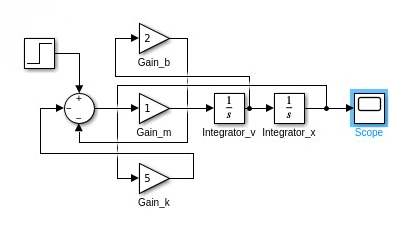
\includegraphics[width=0.7\linewidth]{01.png}
\vspace{0.5cm}

\textbf{Nota:} Esta montagem foi feita automaticamente via código MATLAB, o que demonstra que é possível reproduzir o processo computacionalmente — princípio que será utilizado na criação do app.

Interface MATLAB/Simulink (código, diagrama de blocos e o gráfico simulado):

\vspace{0.5cm}
\centering
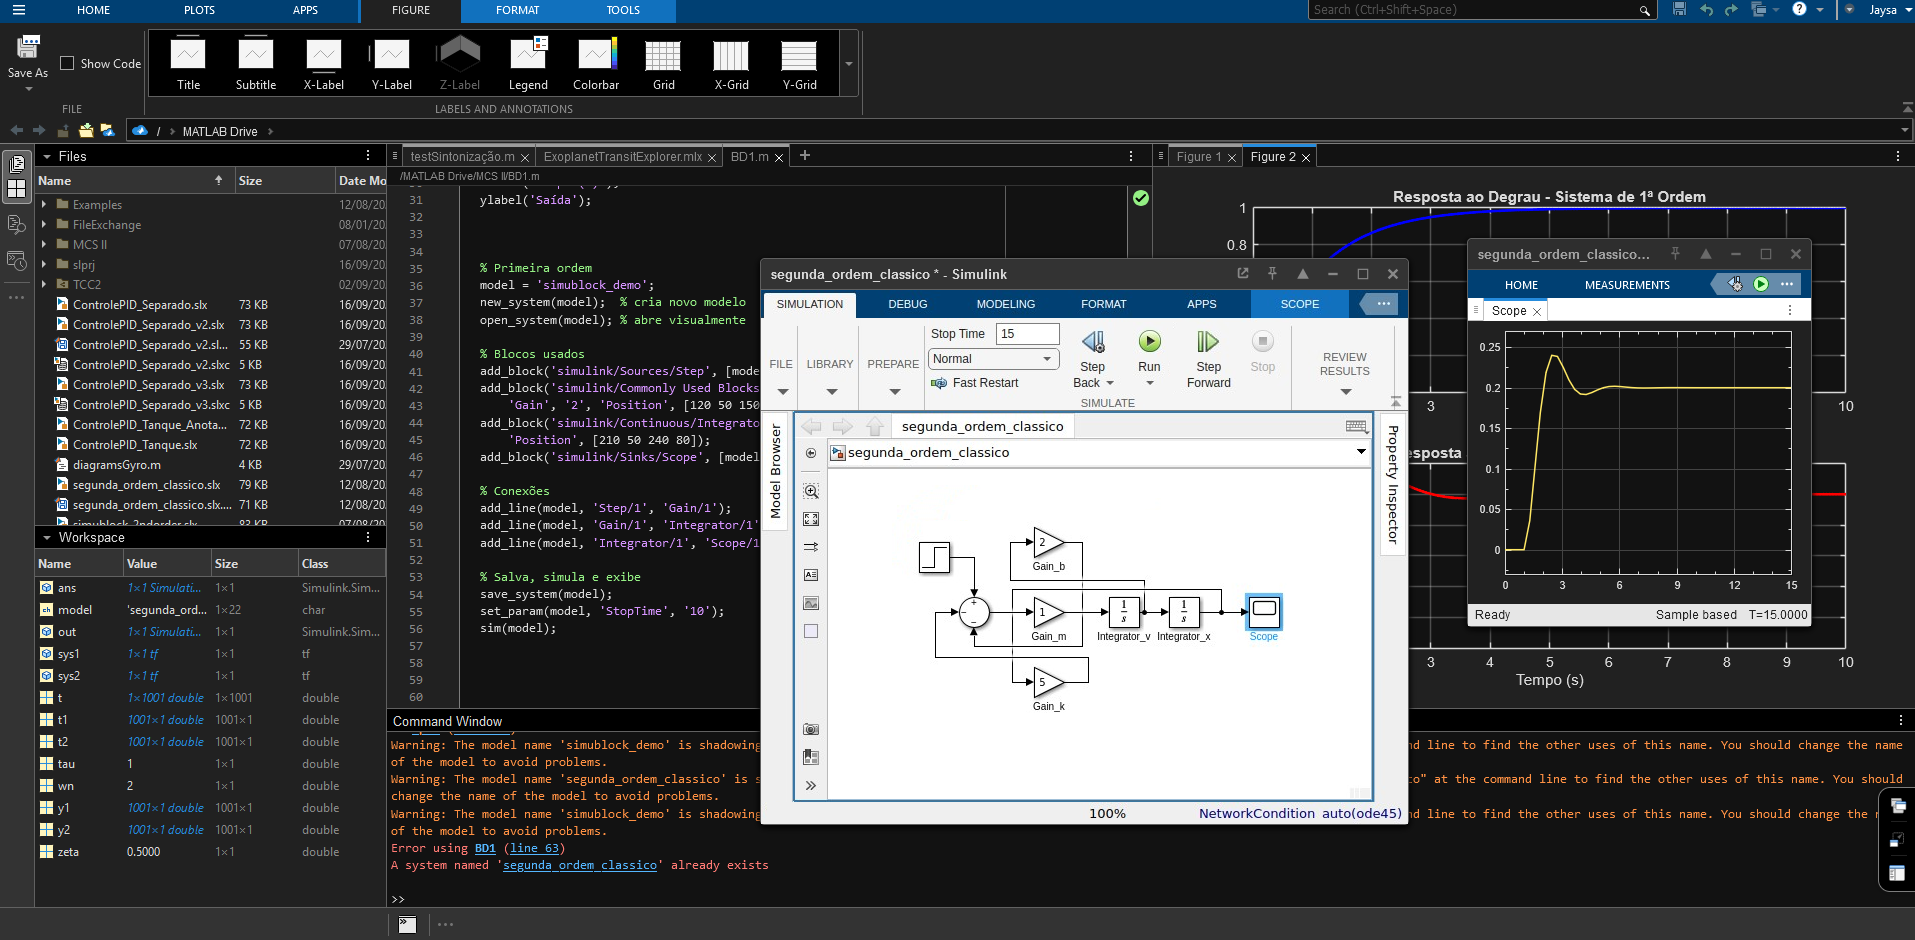
\includegraphics[width=1.0\linewidth]{02.png}
\vspace{0.5cm}

\end{document}
